% Options for packages loaded elsewhere
\PassOptionsToPackage{unicode}{hyperref}
\PassOptionsToPackage{hyphens}{url}
%
\documentclass[
  11pt,
]{article}
\usepackage{amsmath,amssymb}
\usepackage{iftex}
\ifPDFTeX
  \usepackage[T1]{fontenc}
  \usepackage[utf8]{inputenc}
  \usepackage{textcomp} % provide euro and other symbols
\else % if luatex or xetex
  \usepackage{unicode-math} % this also loads fontspec
  \defaultfontfeatures{Scale=MatchLowercase}
  \defaultfontfeatures[\rmfamily]{Ligatures=TeX,Scale=1}
\fi
\ifPDFTeX\else
  % xetex/luatex font selection
\fi
% Use upquote if available, for straight quotes in verbatim environments
\IfFileExists{upquote.sty}{\usepackage{upquote}}{}
\IfFileExists{microtype.sty}{% use microtype if available
  \usepackage[expansion=false]{microtype}
  \UseMicrotypeSet[protrusion]{basicmath} % disable protrusion for tt fonts
}{}
\makeatletter
\@ifundefined{KOMAClassName}{% if non-KOMA class
  \IfFileExists{parskip.sty}{%
    \usepackage{parskip}
  }{% else
    \setlength{\parindent}{0pt}
    \setlength{\parskip}{6pt plus 2pt minus 1pt}}
}{% if KOMA class
  \KOMAoptions{parskip=half}}
\makeatother
\usepackage{xcolor}
\usepackage[margin=1in]{geometry}
\usepackage{longtable,booktabs,array}
\usepackage{calc} % for calculating minipage widths
% Correct order of tables after \paragraph or \subparagraph
\usepackage{etoolbox}
\makeatletter
\patchcmd\longtable{\par}{\if@noskipsec\mbox{}\fi\par}{}{}
\makeatother
% Allow footnotes in longtable head/foot
\IfFileExists{footnotehyper.sty}{\usepackage{footnotehyper}}{\usepackage{footnote}}
\makesavenoteenv{longtable}
\usepackage{graphicx}
\makeatletter
\def\maxwidth{\ifdim\Gin@nat@width>\linewidth\linewidth\else\Gin@nat@width\fi}
\def\maxheight{\ifdim\Gin@nat@height>\textheight\textheight\else\Gin@nat@height\fi}
\makeatother
% Scale images if necessary, so that they will not overflow the page
% margins by default, and it is still possible to overwrite the defaults
% using explicit options in \includegraphics[width, height, ...]{}
\setkeys{Gin}{width=\maxwidth,height=\maxheight,keepaspectratio}
% Set default figure placement to htbp
\makeatletter
\def\fps@figure{htbp}
\makeatother
\setlength{\emergencystretch}{3em} % prevent overfull lines
\providecommand{\tightlist}{%
  \setlength{\itemsep}{0pt}\setlength{\parskip}{0pt}}
\setcounter{secnumdepth}{-\maxdimen} % remove section numbering
\ifLuaTeX
  \usepackage{selnolig}  % disable illegal ligatures
\fi
\IfFileExists{bookmark.sty}{\usepackage{bookmark}}{\usepackage{hyperref}}
\IfFileExists{xurl.sty}{\usepackage{xurl}}{} % add URL line breaks if available
\urlstyle{same}
\hypersetup{
  hidelinks,
  pdfcreator={LaTeX via pandoc}}

\author{}
\date{}

\begin{document}

\textbf{Generative Models vs Traditional AI-Driven Anomaly Detection in
Large-Scale System Logs: A Comparative Study}

Muhammad Asad Mahmood Khan

\emph{Department of Creative Technologies}

\emph{Air University}

\emph{Islamabad, Pakistan}

\emph{asadkhanofficial2341@gmail.com}

\emph{\textbf{Abstract---}The escalating scale and complexity of
distributed computing architectures---Hadoop (HDFS), Apache Spark, and
Hadoop/OpenStack---have rendered manual and rule-based log monitoring
intractable. This paper presents a comparative study evaluating
Traditional Machine Learning (ML), sequence-based Deep Learning (DL),
and Generative AI models for automated anomaly detection in massive,
unstructured log collections. Benchmarking reveals that traditional
supervised algorithms (XGBoost, Random Forest) achieve near-perfect
precision on structured data but rely on labor-intensive manual feature
engineering, while unsupervised baselines such as Isolation Forest
exhibit low efficacy on high-dimensional sequences. Supervised deep
sequence models (LSTM, GRU, CNN) match this accuracy while removing
manual feature extraction, yet degrade sharply under the noise and
concurrency of Spark logs. Generative architectures (LSTM-Autoencoder,
VAE, GAN), trained strictly on normal data, achieve high ROC-AUC but
consistently lower F1-scores, offering a baseline capability for
zero-day anomaly discovery rather than outright superiority. Models were
independently trained and tested within isolated dataset boundaries
(HDFS, Spark, Hadoop) to avoid cross-system contamination. Results
confirm that Traditional ML and supervised Deep Learning outperform
Generative AI across all evaluated datasets, while highlighting
precision trade-offs in highly concurrent environments such as Spark.}

\emph{\textbf{Index Terms---}anomaly detection, system logs, machine
learning, deep learning, generative AI, LSTM, variational autoencoder,
generative adversarial network, HDFS, Apache Spark}

\textsc{I. INTRODUCTION}

System logs are the primary source of truth for diagnosing failures,
tracking execution flow, and ensuring security in modern cloud
infrastructures. In distributed computing paradigms such as the Hadoop
Distributed File System (HDFS) and Apache Spark, a single transaction
can cascade into execution traces spanning thousands of concurrent
nodes, generating terabytes of heterogeneous, unstructured log data.

Manual inspection and static, rule-based heuristics have become
fundamentally obsolete given this scale. Consequently, the industry has
shifted toward Artificial Intelligence---spanning Traditional Machine
Learning (ML), Deep Learning (DL), and Generative AI---to parse, embed,
and analyze massive log collections for automated anomaly detection.

\emph{A. Problem Statement}

Current industry standards for automated log anomaly detection are
paralyzed by a dichotomy between accuracy and adaptability. Supervised
models such as SVM and XGBoost achieve high accuracy in closed-world
scenarios but depend on rigid manual feature engineering (e.g., Event
Count Matrices) and labeled datasets, failing under concept drift.
Unsupervised baselines (Isolation Forest, One-Class SVM) avoid labeling
requirements but struggle to capture temporal and sequential
dependencies, producing high false-positive rates and poor detection of
unknown, zero-day errors. A unified framework combining supervised
accuracy with unsupervised flexibility remains absent.

\emph{B. Objectives and Research Questions}

This research benchmarks Traditional ML, sequence-based DL, and
Generative AI on HDFS, Spark, and Hadoop datasets, producing a tri-fold
comparative performance matrix. The core research questions are:

RQ1: To what extent can Generative AI maintain consistent anomaly
detection performance across heterogeneous distributed systems compared
to Traditional Supervised models?

RQ2: Can Generative Deep Learning eliminate the dependency on manual
feature engineering while maintaining high F1-scores?

RQ3: Can deep generative models significantly outperform traditional
unsupervised baselines in detecting unknown zero-day anomaly patterns?

\textsc{II. LITERATURE SURVEY}

\emph{A. Traditional Machine Learning}

Foundational log anomaly detection studies relied on supervised
algorithms such as Decision Trees, SVM, Random Forest, and XGBoost,
achieving high accuracy on structured, well-balanced datasets after
parsing raw logs into fixed templates (e.g., using Drain {[}3{]}) and
constructing Event Count Matrices or TF-IDF features. These
discriminative models are brittle: a shift in log syntax or system
architecture can catastrophically degrade performance. Unsupervised
baselines such as Isolation Forest {[}7{]} mitigate the need for labeled
data but struggle with high-dimensional sequential data, producing high
false-positive rates.

\emph{B. Deep Learning Sequence Models}

To address manual feature engineering, DeepLog {[}4{]} modeled system
logs as natural-language sequences using LSTM networks, learning normal
patterns and detecting anomalies as deviations, outperforming
traditional data-mining methods. LogAnomaly {[}2{]} extended this by
integrating sequential and semantic log information. CNN-based spatial
models have also been adapted to detect local anomalies within log
windows. These supervised DL models remain vulnerable to the
out-of-vocabulary problem, where unseen log events cause
misclassification of normal operations.

\emph{C. Generative and Transformer Models}

Recent work leverages self-supervised and Transformer-based
architectures such as LogBERT to capture contextual relationships
between log events. Generative architectures---VAEs, GANs (e.g.,
LogGAN), and LSTM-Autoencoders---are trained exclusively on normal
operational data, flagging anomalies via reconstruction error or
probabilistic deviation. While these models theoretically remove
dependency on labeled data and feature engineering, they are
computationally expensive and sensitive to reconstruction thresholds,
degrading in highly concurrent, noisy environments such as Apache Spark.

\emph{D. Research Gap}

Most existing studies evaluate models under isolated, single-dataset
benchmarks (typically HDFS), which fails to reflect complex enterprise
environments. Comprehensive, multi-source comparative research
subjecting Traditional ML, DL, and Generative AI to identical conditions
across structurally distinct datasets---HDFS, Spark, and
Hadoop---remains lacking, leaving the trade-off between accuracy and
architectural autonomy largely unresolved.

\textsc{III. MATHEMATICAL FORMULATION}

Raw, unstructured logs are parsed into structured event templates. A
parsed log sequence of length T is defined as an ordered set of log
events:

\emph{E = \{e1, e2, \ldots, eT\}} (1)

where each event et ∈ Rd is a d-dimensional embedding of the log event
at time step t, bypassing manual Event Count Matrices.

For sequence modeling, an LSTM network updates its hidden state ht from
event et and prior state ht−1, predicting the probability of the next
event among vocabulary V:

\emph{P(et+1 = vi \textbar{} e1,\ldots,et) = exp(Wi ht + bi) / Σj exp(Wj
ht + bj)} (2)

Generative models are trained strictly on normal sequences within
isolated dataset boundaries. A Variational Autoencoder (VAE) learns the
underlying distribution of normal sequences by optimizing the Evidence
Lower Bound (ELBO):

\emph{LVAE = −Eqϕ(z\textbar x){[}log pθ(x\textbar z){]} +
DKL(qϕ(z\textbar x) ‖ p(z))} (3)

where x is the input log sequence, z the latent representation,
qϕ(z\textbar x) the encoder, pθ(x\textbar z) the decoder, and DKL the
Kullback--Leibler divergence regularizer.

At test time, an anomaly score A(x) is computed from the reconstruction
loss; an anomaly is flagged when this loss exceeds a dynamic threshold
τ:

\emph{A(x) = ‖x − pθ(x\textbar z)‖² \textgreater{} τ} (4)

\textsc{IV. METHODOLOGY}

The study follows a five-phase comparative methodology (Fig. 1),
independently training and testing all models within isolated dataset
boundaries (HDFS, Spark, Hadoop) to avoid cross-system contamination.

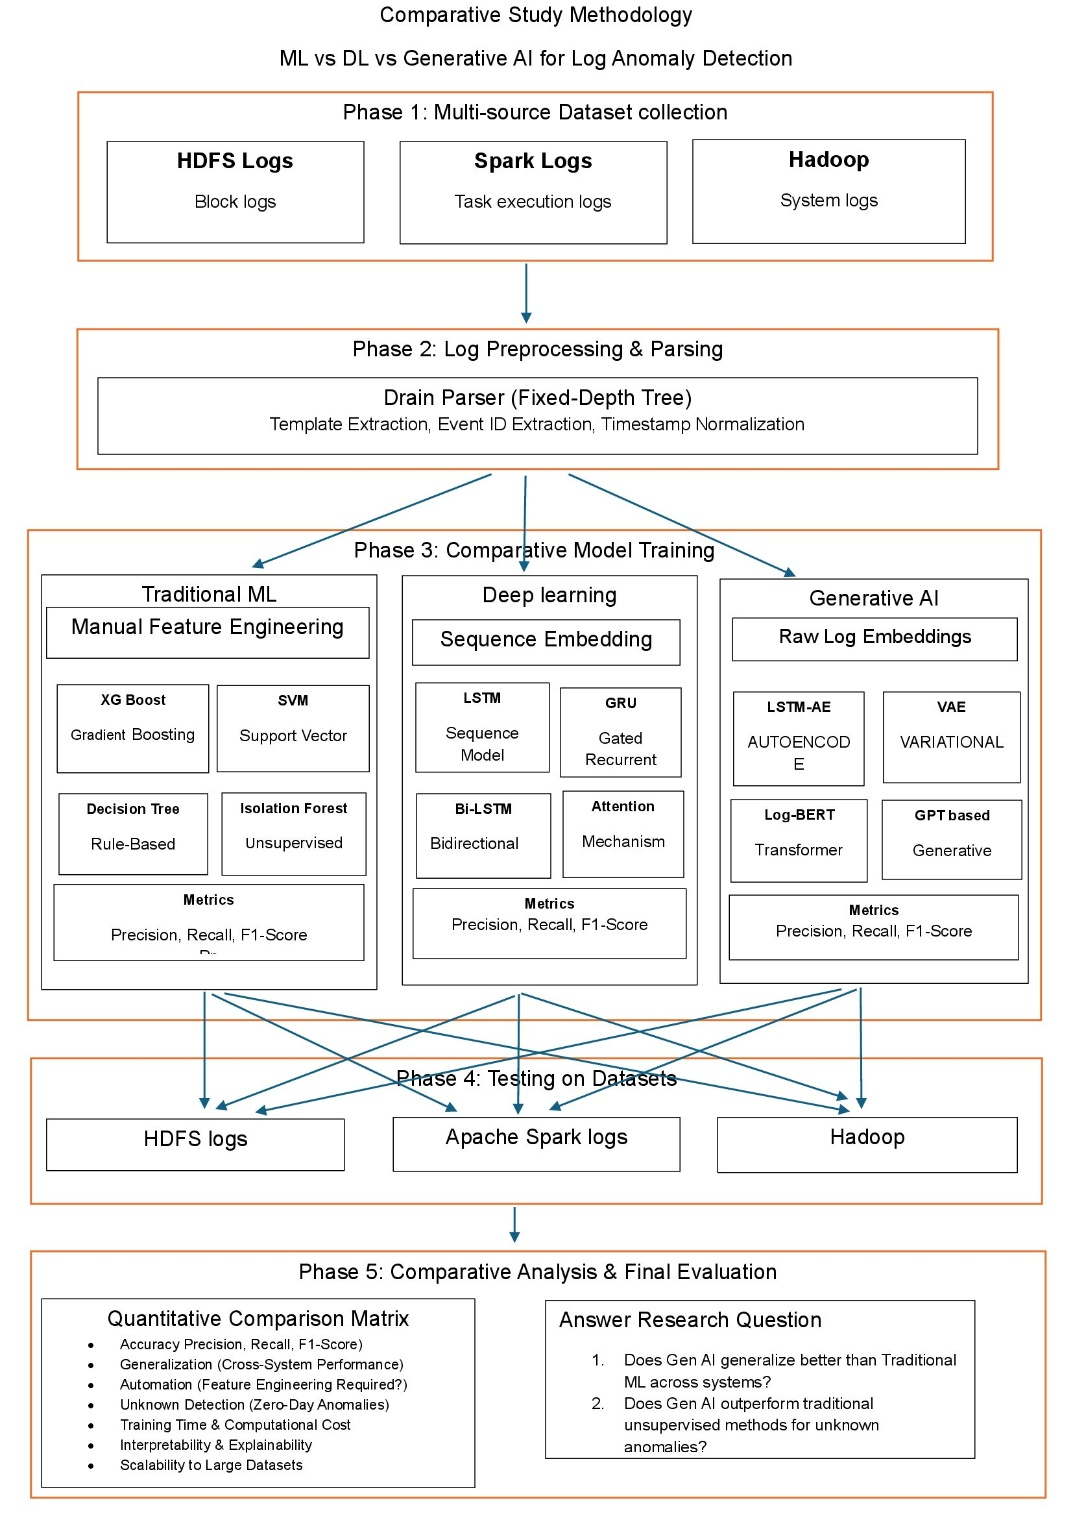
\includegraphics[width=2.96875in,height=4.19792in]{./media/2f3c9ab99b17edec963cb493396b605ade69c150.png}

Fig. 1. Five-phase comparative study methodology.

\emph{A. Phase 1 -- Multi-Source Dataset Collection}

HDFS block logs, Apache Spark task execution logs, and Hadoop system
logs form a multi-source repository for heterogeneous comparative
testing.

\emph{B. Phase 2 -- Log Preprocessing and Parsing}

Raw logs are processed with the Drain parser {[}3{]}, a fixed-depth tree
approach, performing template extraction, event ID extraction, and
timestamp normalization.

\emph{C. Phase 3 -- Comparative Model Architectures}

Three parallel pipelines are implemented: (i) Traditional ML (XGBoost,
Random Forest, Isolation Forest) using Event Count Matrices; (ii) Deep
Learning sequence models (LSTM, GRU, Bi-LSTM with attention, CNN)
operating directly on log sequences; and (iii) Generative AI (VAE, GAN,
LSTM-Autoencoder) trained on normal-only data using raw log embeddings,
with anomaly scores derived from reconstruction probability.

\emph{D. Phase 4 -- Training and Testing Dynamics}

Each model is evaluated with an 80/20 train-test split sourced from the
same dataset (intra-system validation), independently repeated across
HDFS, Spark, and Hadoop to verify performance consistency without
cross-contaminating training distributions.

\emph{E. Phase 5 -- Comparative Analysis}

Models are assessed via Precision, Recall, F1-score, ROC-AUC, and
PR-AUC, alongside qualitative criteria: performance consistency,
automation level, zero-day detection capability, training time,
interpretability, and scalability.

\textsc{V. RESULTS AND DISCUSSION}

\emph{A. HDFS Baseline Performance}

Models were evaluated on an 80/20 split of the HDFS dataset (558,223
normal, 16,838 anomaly log vectors; 115,013-instance test set). XGBoost
achieved near-perfect performance, with 5 false positives and 1 missed
anomaly out of 3,368.

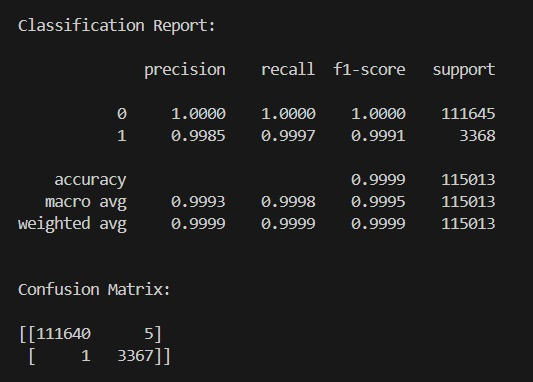
\includegraphics[width=3.125in,height=2.23958in]{./media/2e2476b7371b6938231aa0b67cfc4504057a8dc7.png}

Fig. 2. HDFS ML XGBoost confusion matrix.

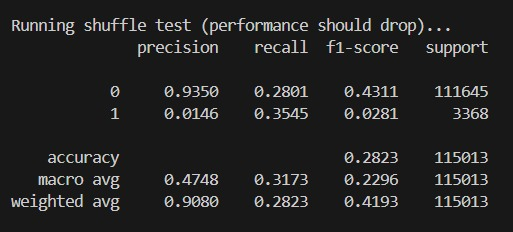
\includegraphics[width=3.125in,height=1.41667in]{./media/138dc130ee0869c9c9b78ff00bae65fd5d5f24e0.png}

Fig. 3. XGBoost shuffling-test performance.

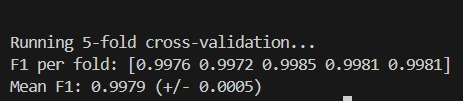
\includegraphics[width=3.125in,height=0.67708in]{./media/ffc99b85061ae9a226c37a69c055f0034e77705b.png}

Fig. 4. XGBoost F1-score summary.

SVM achieved strong baseline performance (128 false positives, 2 missed
anomalies), though XGBoost outperformed it across all key parameters,
reflecting its superior capacity for non-linear decision boundaries.

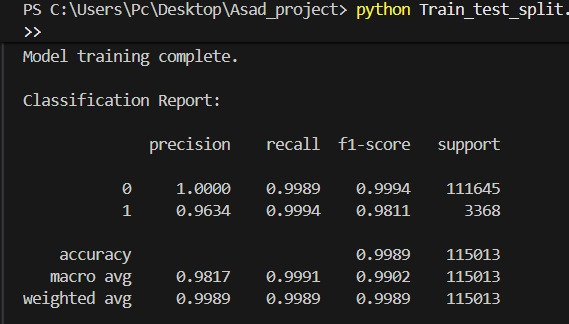
\includegraphics[width=3.125in,height=1.78125in]{./media/65ef54c2c61cc167677caaf6ff1aa93b142ee3b6.png}

Fig. 5. SVM results on HDFS.

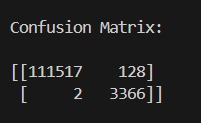
\includegraphics[width=2.34375in,height=1.4375in]{./media/d35701f94fdfb3c42cc8e66affb47f3eefb29c99.png}

Fig. 6. SVM confusion matrix.

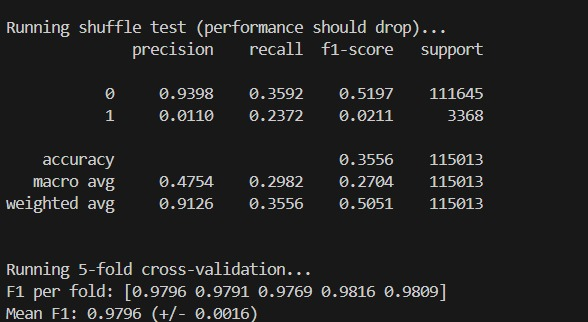
\includegraphics[width=3.125in,height=1.70833in]{./media/0e1fd968d69e674598eaccb37caf999c3e1778a0.png}

Fig. 7. SVM results after shuffling.

The supervised Deep Learning pipeline evaluated sequence models without
rigid manual feature engineering. LSTM produced 66 false positives and
missed 4 anomalies (ROC-AUC = 1.0); GRU performed comparably, missing
only 3 anomalies.

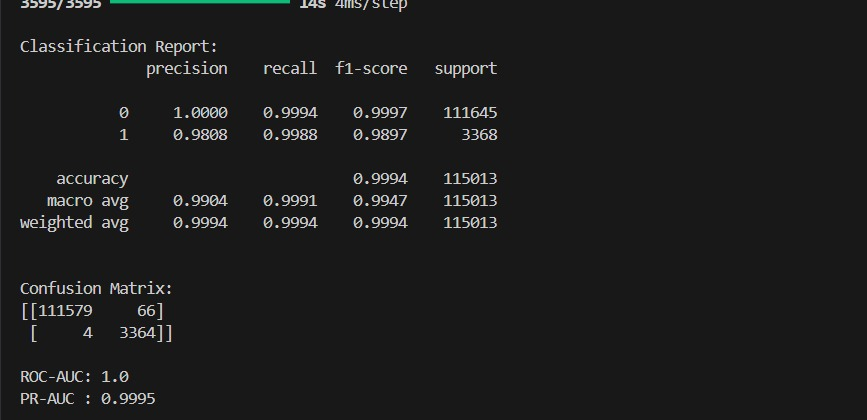
\includegraphics[width=3.125in,height=1.51042in]{./media/baadb35db958ee3c0d4f4b3d70701c1eab3b62cd.png}

Fig. 8. DL LSTM confusion matrix and ROC-AUC results.

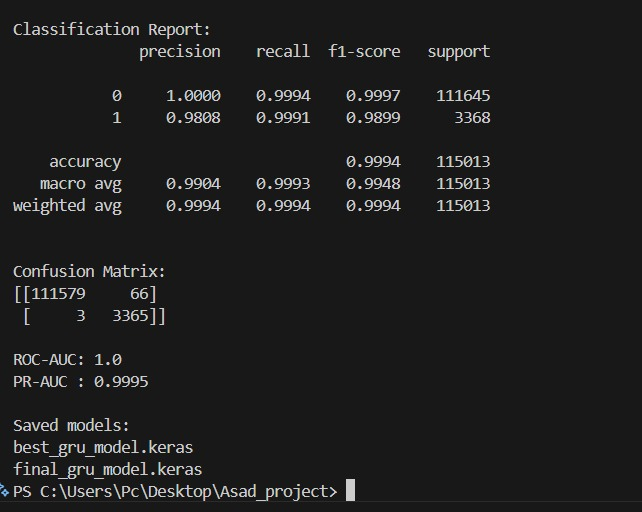
\includegraphics[width=3.125in,height=2.48958in]{./media/8dbcfcaba08f5a883f1b9f27309d2ac357bb1c4c.png}

Fig. 9. GRU confusion matrix and ROC-AUC results.

Generative AI models were trained exclusively on normal sequences. The
LSTM-Autoencoder produced 1,137 false positives and 398 missed anomalies
(ROC-AUC 0.9964, PR-AUC 0.9049); the LSTM-VAE produced 1,101 false
positives and 866 missed anomalies (ROC-AUC 0.9876, PR-AUC 0.7854).

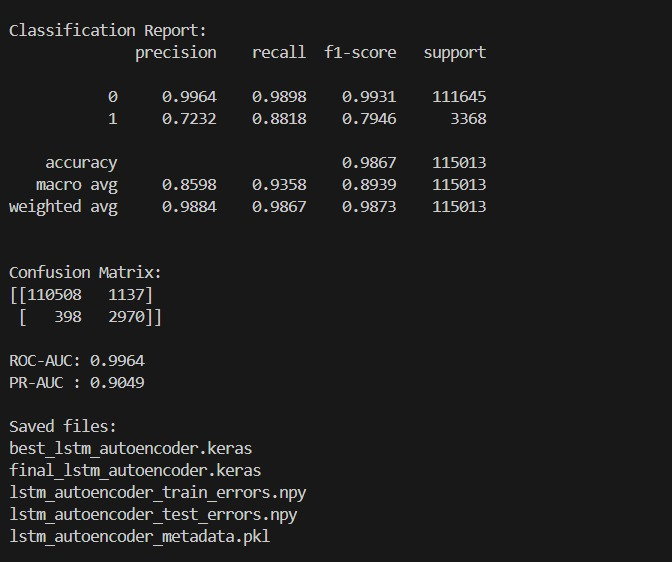
\includegraphics[width=3.125in,height=2.61458in]{./media/13ae6bfd4fc44aa743c58d6286f70abf36059e88.png}

Fig. 10. Generative AI LSTM-Autoencoder confusion matrix and ROC-AUC
results.

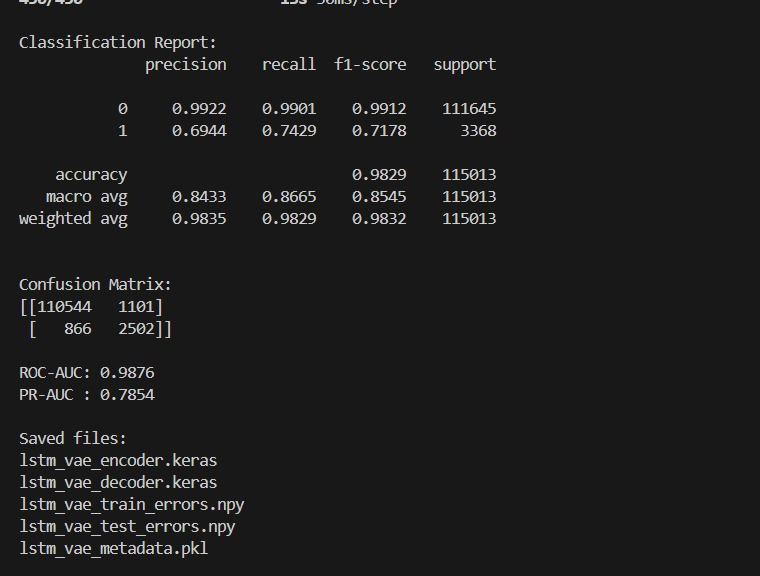
\includegraphics[width=3.125in,height=2.36458in]{./media/cbcfd242ac0121b446dc28b82477e47bc23a9380.png}

Fig. 11. Generative AI LSTM-VAE confusion matrix and ROC-AUC results.

Table I and Fig. 12 summarize the HDFS comparison: XGBoost and the
supervised DL models (LSTM, GRU) dominate, while generative models
establish a lower, but non-trivial, zero-day detection baseline.

TABLE I\\
HDFS MODEL COMPARISON

\begin{longtable}[]{@{}
  >{\raggedright\arraybackslash}p{(\columnwidth - 10\tabcolsep) * \real{0.1915}}
  >{\raggedright\arraybackslash}p{(\columnwidth - 10\tabcolsep) * \real{0.1809}}
  >{\raggedright\arraybackslash}p{(\columnwidth - 10\tabcolsep) * \real{0.1596}}
  >{\raggedright\arraybackslash}p{(\columnwidth - 10\tabcolsep) * \real{0.1596}}
  >{\raggedright\arraybackslash}p{(\columnwidth - 10\tabcolsep) * \real{0.1596}}
  >{\raggedright\arraybackslash}p{(\columnwidth - 10\tabcolsep) * \real{0.1489}}@{}}
\toprule\noalign{}
\endhead
\bottomrule\noalign{}
\endlastfoot
\textbf{Model} & \textbf{Type} & \textbf{Prec.} & \textbf{Recall} &
\textbf{F1} & \textbf{ROC-AUC} \\
XGBoost & Trad. ML & 99.85\% & 99.97\% & 99.91\% & -- \\
SVM & Trad. ML & 96.34\% & 99.94\% & 98.11\% & -- \\
LSTM & Sup. DL & 98.08\% & 99.88\% & 98.97\% & 100.0\% \\
GRU & Sup. DL & 98.08\% & 99.91\% & 98.99\% & 100.0\% \\
LSTM-AE & Generative & 72.32\% & 88.18\% & 79.46\% & 99.64\% \\
LSTM-VAE & Generative & 69.44\% & 74.29\% & 71.78\% & 98.76\% \\
\end{longtable}

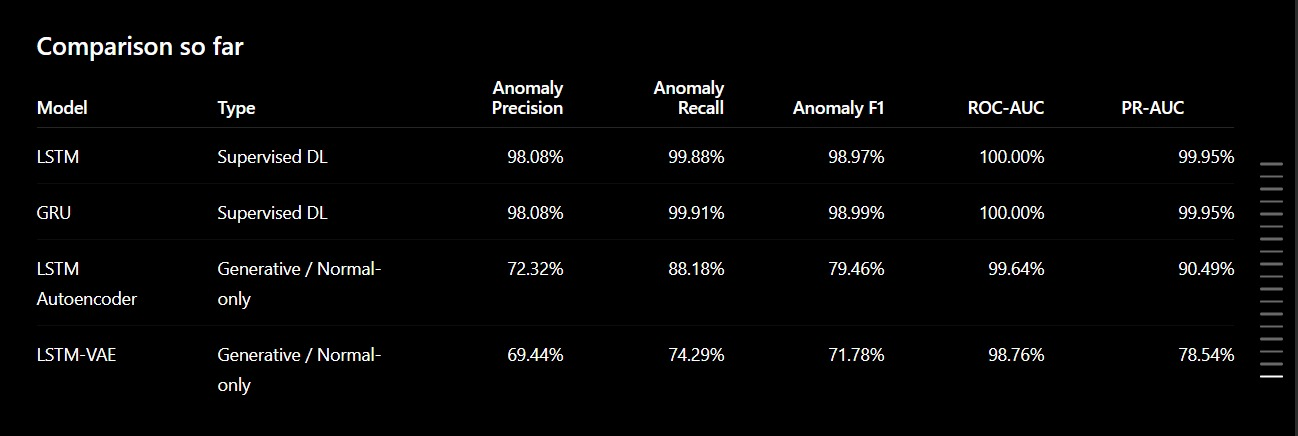
\includegraphics[width=3.125in,height=1.05208in]{./media/734899353cbdfe69e8ff45b100a26c4a81fe8087.png}

Fig. 12. HDFS comparison matrix across all evaluated models.

\emph{B. Spark Logs Analysis}

On Apache Spark logs, Random Forest achieved the strongest ROC-AUC
(0.9902), while Isolation Forest (0.9559) and One-Class SVM (0.2388)
performed poorly; Isolation Forest also suffered low precision and F1
(0.04).

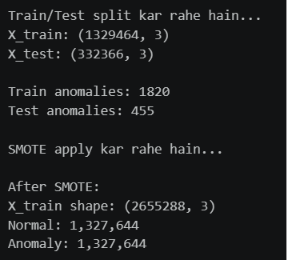
\includegraphics[width=2.65625in,height=2.40625in]{./media/c217a5f0e2df14322ae2d118150663fa20c72ac3.png}

Fig. 13. Spark ML train and test results.

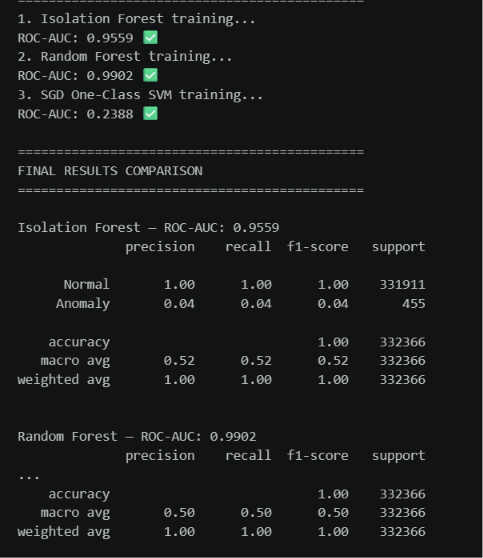
\includegraphics[width=2.96875in,height=3.42708in]{./media/24eb75c614d5a9728918352a68f9153cbedaa878.png}

Fig. 14. Isolation Forest and Random Forest results.

The LSTM-Autoencoder reached ROC-AUC 0.9822 with recall 0.93 for
anomalies, but precision of only 0.02 (F1 = 0.05), reflecting severe
false-positive volume.

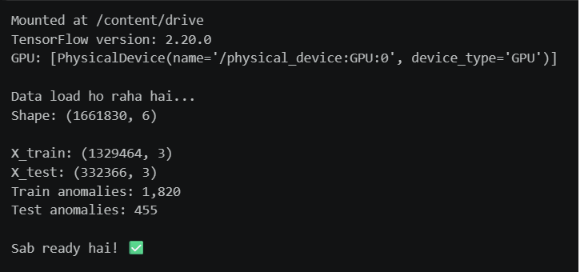
\includegraphics[width=3.125in,height=1.46875in]{./media/84bf07d3d99e9b4029f233ea9eddd5acfe1d7e22.png}

Fig. 15. Deep Learning train and test results (Spark).

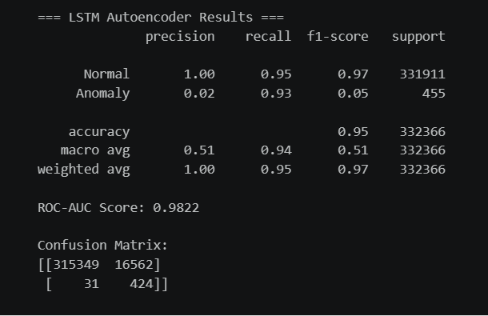
\includegraphics[width=3.125in,height=2.02083in]{./media/35930f2015c925f2a2e3bb2d80d2b9489c19010c.png}

Fig. 16. LSTM results (Spark).

The CNN classifier recorded the highest overall ROC-AUC (0.9978) with
perfect recall (1.00), but likewise suffered severe precision collapse
(0.09), yielding F1 = 0.16.

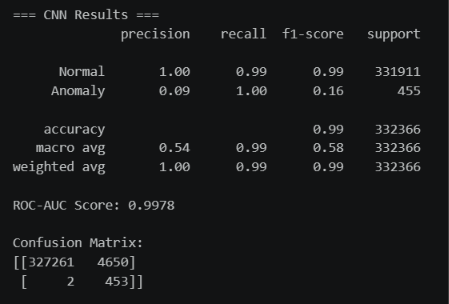
\includegraphics[width=3.125in,height=2.11458in]{./media/b8a71891948e100c3f5cbca481bb964b683bbbaa.png}

Fig. 17. CNN results (Spark).

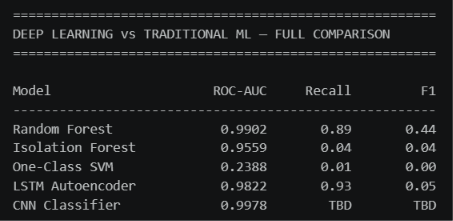
\includegraphics[width=3.125in,height=1.52083in]{./media/ce40c0cac57eddb6e5b46ba5cb2087b350d0116d.png}

Fig. 18. Deep Learning vs Traditional ML comparison (Spark).

Both generative models performed poorly on Spark: the VAE reached
ROC-AUC 0.7700 with F1 = 0.01, while the GAN failed to detect anomalies
effectively (ROC-AUC 0.2479, F1 = 0.01).

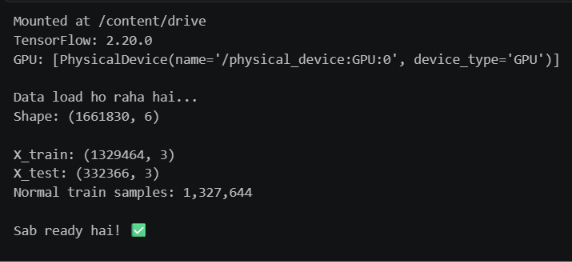
\includegraphics[width=3.125in,height=1.42708in]{./media/7c36c8cf8c53570b689970bea5cc3b627e46b8e3.png}

Fig. 19. Generative AI train and test results (Spark).

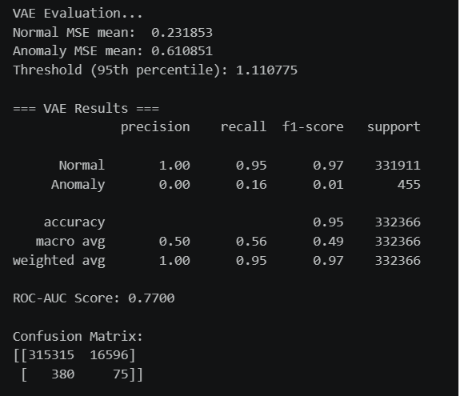
\includegraphics[width=3.125in,height=2.69792in]{./media/e8cfae8e44dd57006f65ca740a323a622f14c100.png}

Fig. 20. VAE results (Spark).

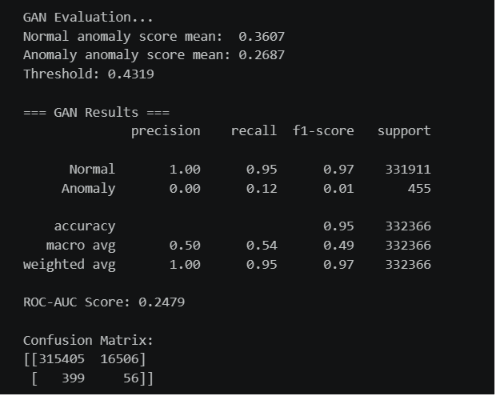
\includegraphics[width=3.125in,height=2.48958in]{./media/d75874d8ff20e02f5cac84901b615a988dd6ca44.png}

Fig. 21. GAN results (Spark).

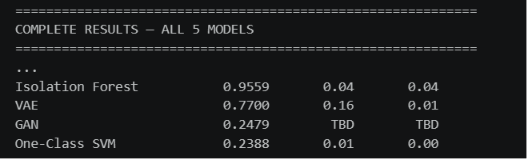
\includegraphics[width=3.125in,height=0.94792in]{./media/52a7fd8f75e73657cd50f3f363de408c3d755099.png}

Fig. 22. Generative model summary panel (Spark).

Spark Comparative Analysis Synthesis

The complex, overlapping nature of Spark execution logs created a
massive false-positive problem: the LSTM-Autoencoder alone generated
16,562 false positives, dropping F1 to 0.05 despite a strong ROC-AUC of
0.9822. Both generative models collapsed to F1 = 0.01, indicating that
Spark\textquotesingle s structural noise and concurrency fundamentally
disrupt latent-distribution mapping.

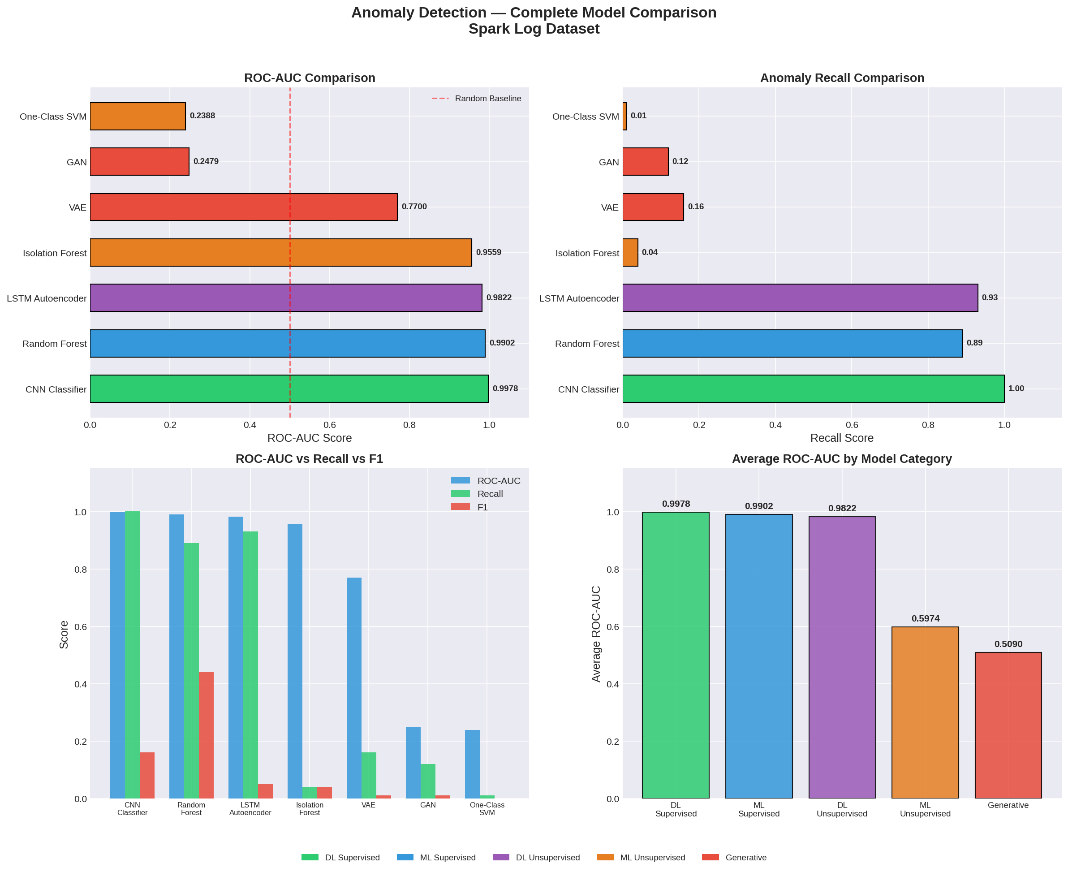
\includegraphics[width=3.125in,height=2.55208in]{./media/2e98b7dd650a6896a48750d937bf65a20bfe6061.png}

Fig. 23. Spark logs model comparison.

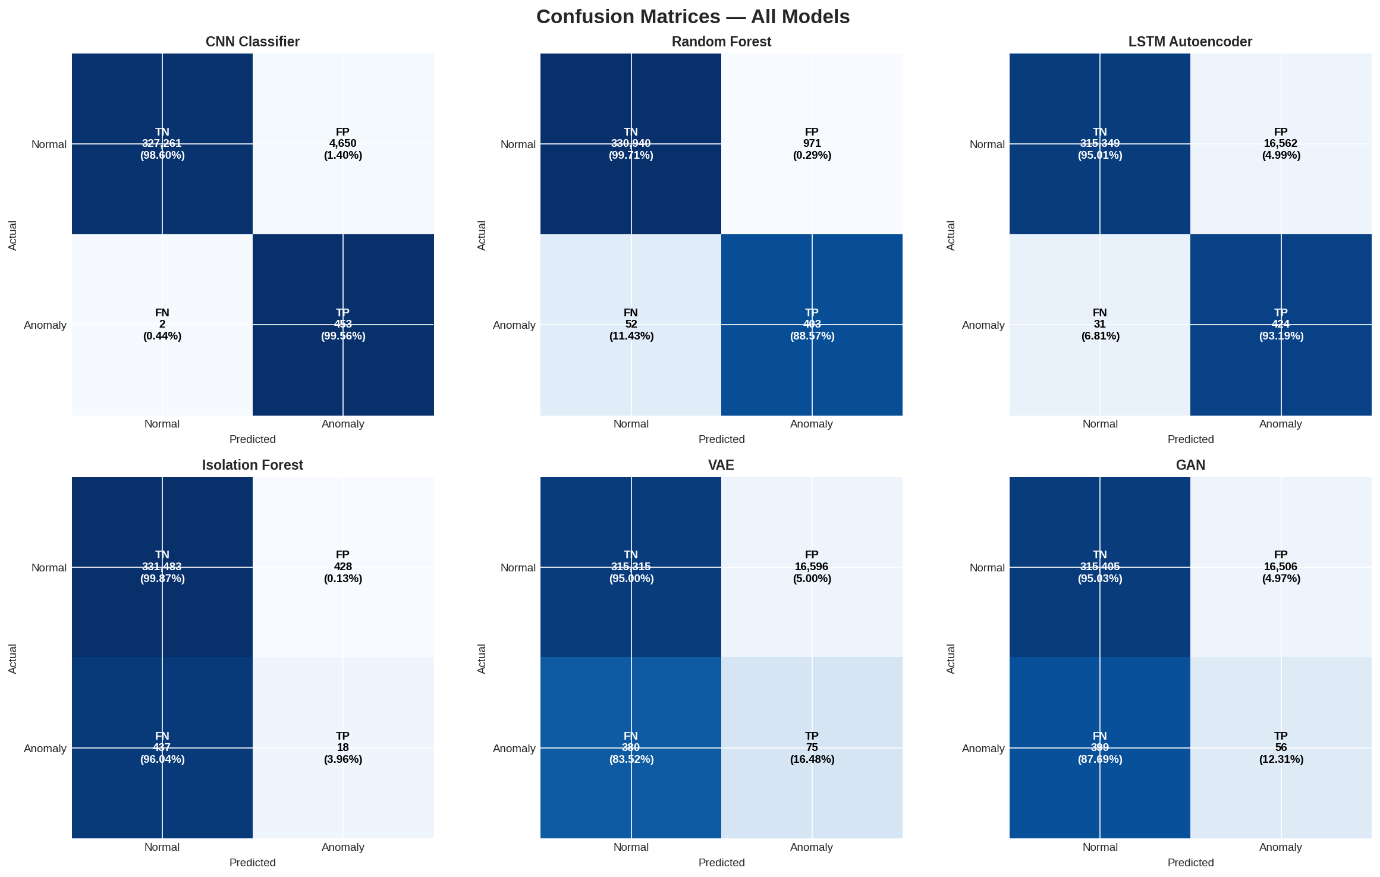
\includegraphics[width=3.125in,height=1.98958in]{./media/209fa0024a5fc719862a539587492cf4f303856d.png}

Fig. 24. Spark logs confusion matrix.

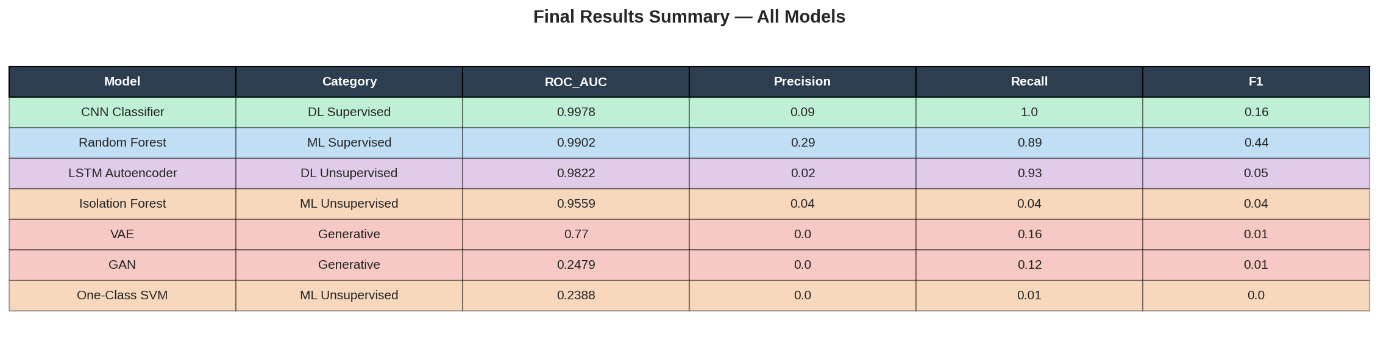
\includegraphics[width=3.125in,height=0.77083in]{./media/7741142afc84df749d904a4886d6e204a8029a04.png}

Fig. 25. Spark logs comparative summary.

\emph{C. Hadoop Logs Analysis}

On Hadoop, Random Forest achieved perfect metrics (ROC-AUC, Recall, F1 =
1.0000); this is attributable to per-application label leakage rather
than genuine separability, making the Spark results more reliable for
cross-dataset comparison. Isolation Forest and One-Class SVM performed
poorly (ROC-AUC 0.2092 and 0.2383).

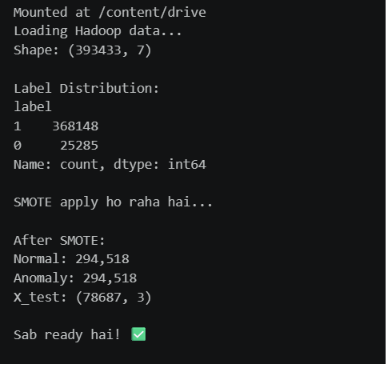
\includegraphics[width=2.8125in,height=2.65625in]{./media/3dd67acb7a3fbb857176e855cfe06f4979b053a3.png}

Fig. 26. Hadoop ML label-logs distribution.

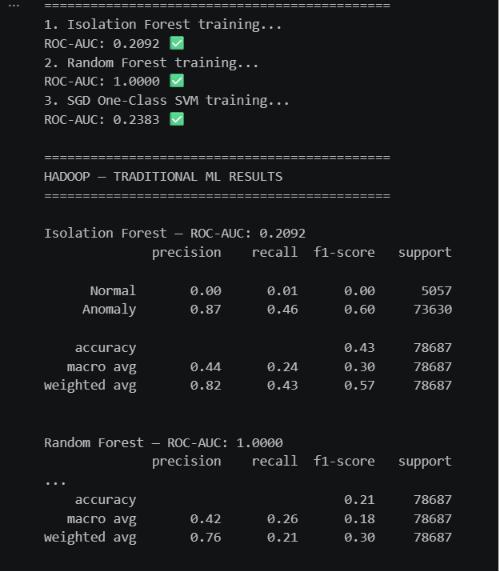
\includegraphics[width=2.96875in,height=3.40625in]{./media/c9108a555eccabdbacceaaf41d048c16d85a2060.png}

Fig. 27. ML Isolation Forest and Random Forest results (Hadoop).

Deep learning performance was mixed on Hadoop. The CNN classifier
performed strongly (ROC-AUC 0.9617, F1 = 0.91); the LSTM-Autoencoder
degraded sharply relative to its Spark result (ROC-AUC 0.6519, F1 =
0.45).

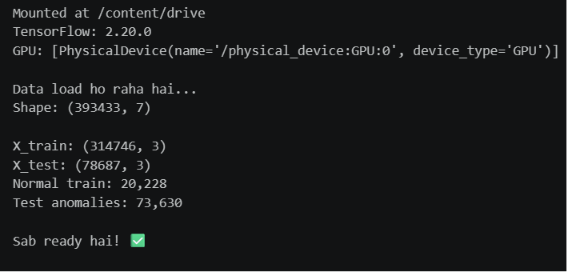
\includegraphics[width=3.125in,height=1.5in]{./media/d26f55b5b2c1b8c16afb4dde94d04485ff67eb29.png}

Fig. 28. Deep Learning train/test results (Hadoop).

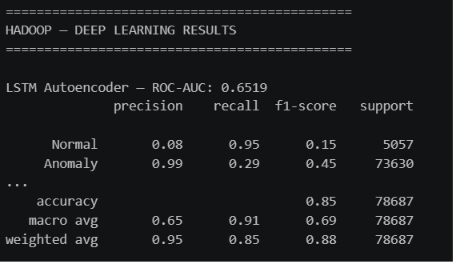
\includegraphics[width=3.125in,height=1.8125in]{./media/ff1451c95cebc57f0183bc43d8097f7568cac27a.png}

Fig. 29. LSTM-Autoencoder results (Hadoop).

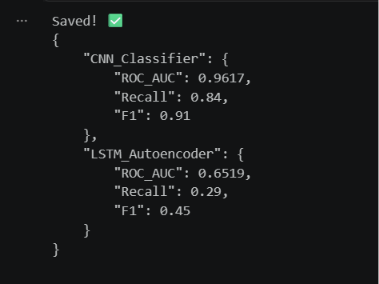
\includegraphics[width=2.65625in,height=1.98958in]{./media/cc871190cc5f60d04e4308b5f71083ff4c92841a.png}

Fig. 30. CNN and LSTM comparison (Hadoop).

Generative models remained weak on Hadoop: the GAN achieved ROC-AUC
0.6133 (F1 = 0.03), while the VAE recorded ROC-AUC 0.5235 (F1 = 0.12).

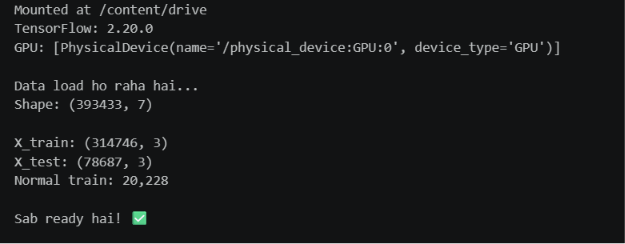
\includegraphics[width=3.125in,height=1.21875in]{./media/9a0a95da6d291ae48326b23db81f72331303d0fd.png}

Fig. 31. Generative AI train/test results (Hadoop).

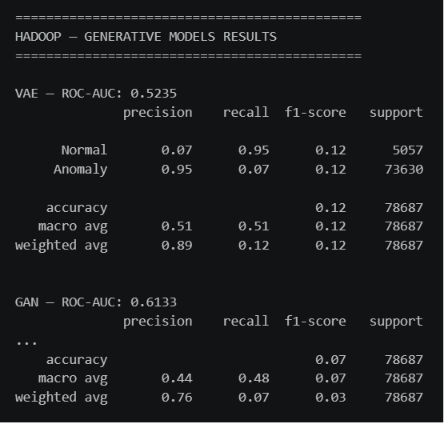
\includegraphics[width=2.96875in,height=2.83333in]{./media/f4d992793d520c437617b78d67ee49fef23dc95d.png}

Fig. 32. VAE and GAN results (Hadoop).

The summary confirms Random Forest\textquotesingle s absolute
superiority on Hadoop, recording zero false positives and zero false
negatives; the CNN also demonstrated high accuracy with only 50 false
positives among tens of thousands of records.

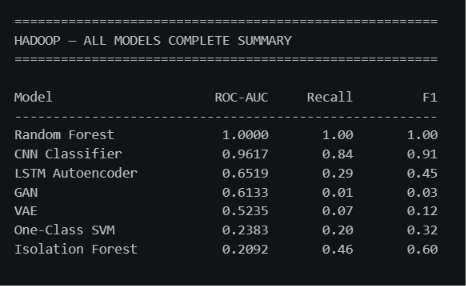
\includegraphics[width=3.125in,height=1.91667in]{./media/9bbb6db67ea29b103fefb702d09dfb52fc9be0c5.png}

Fig. 33. Hadoop --- all-model results summary.

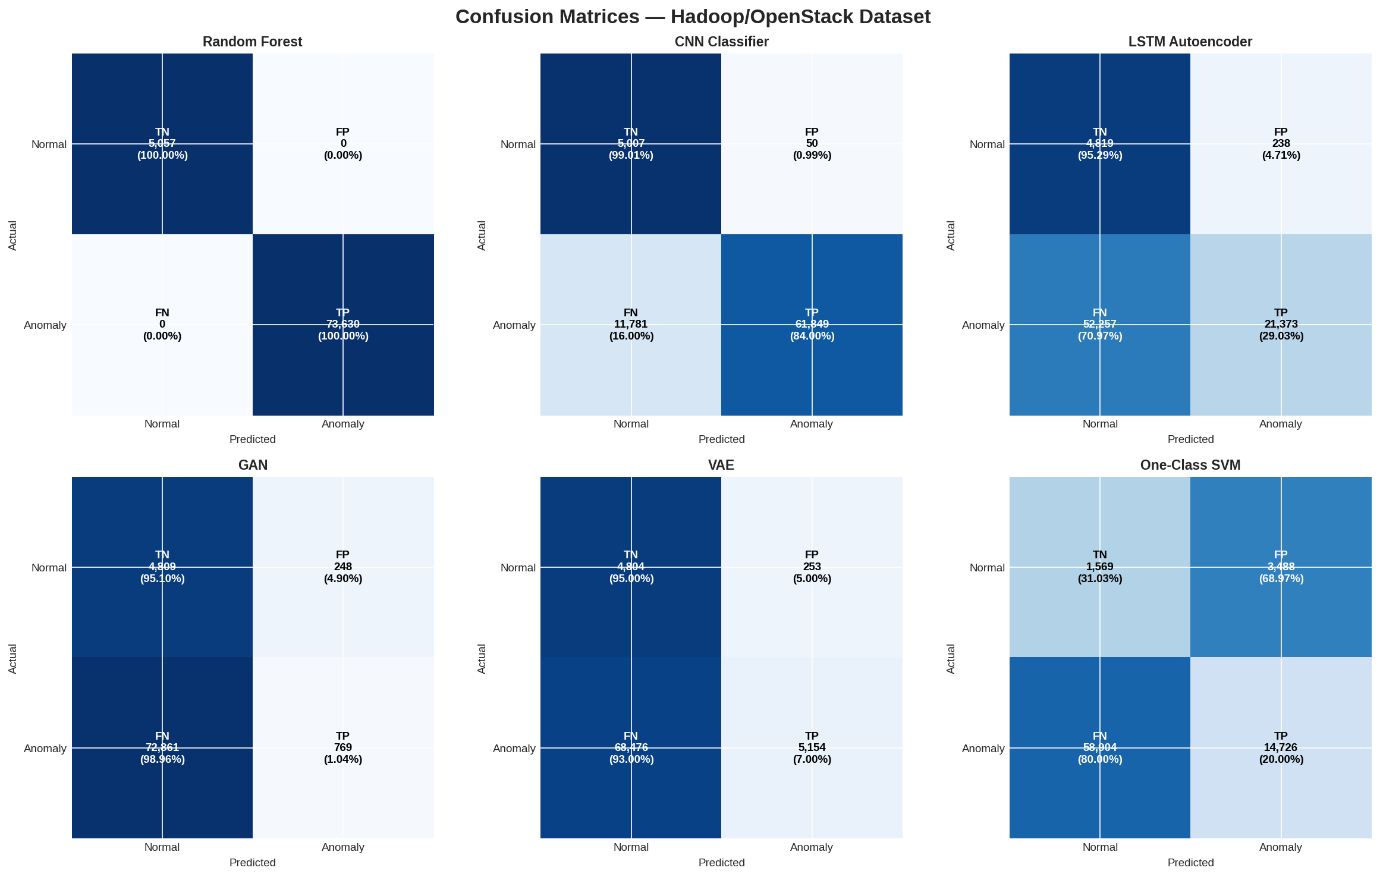
\includegraphics[width=3.125in,height=1.98958in]{./media/48bdcc3ae9b7d750a95fc476dc4689799f3415c4.png}

Fig. 34. Hadoop --- all-model confusion matrix.

\emph{D. Overall Performance Synthesis}

Table II summarizes F1-scores across all three datasets. Random Forest
is the most consistently reliable model overall; CNN shows excellent
ROC-AUC but highly dataset-dependent F1 (0.16 on Spark vs. 0.91 on
Hadoop); Generative and unsupervised models remain consistently weak
across environments.

TABLE II\\
OVERALL MODEL F1-SCORES ACROSS DATASETS

\begin{longtable}[]{@{}
  >{\raggedright\arraybackslash}p{(\columnwidth - 8\tabcolsep) * \real{0.2447}}
  >{\raggedright\arraybackslash}p{(\columnwidth - 8\tabcolsep) * \real{0.2447}}
  >{\raggedright\arraybackslash}p{(\columnwidth - 8\tabcolsep) * \real{0.1702}}
  >{\raggedright\arraybackslash}p{(\columnwidth - 8\tabcolsep) * \real{0.1702}}
  >{\raggedright\arraybackslash}p{(\columnwidth - 8\tabcolsep) * \real{0.1702}}@{}}
\toprule\noalign{}
\endhead
\bottomrule\noalign{}
\endlastfoot
\textbf{Model} & \textbf{Category} & \textbf{HDFS} & \textbf{Spark} &
\textbf{Hadoop} \\
XGBoost & Trad. ML (S) & 0.9991 & -- & -- \\
SVM & Trad. ML (S) & 0.9811 & -- & -- \\
Random Forest & Trad. ML (S) & -- & 0.44 & 1.00 \\
LSTM & DL (Sup.) & 0.9897 & -- & -- \\
GRU & DL (Sup.) & 0.9899 & -- & -- \\
CNN & DL (Sup.) & -- & 0.16 & 0.91 \\
Isolation Forest & Trad. ML (U) & -- & 0.04 & 0.60 \\
One-Class SVM & Trad. ML (U) & -- & 0.00 & 0.32 \\
LSTM-AE & Generative & 0.7946 & 0.05 & 0.45 \\
VAE & Generative & 0.7178 & 0.01 & 0.12 \\
GAN & Generative & -- & 0.01 & 0.03 \\
\end{longtable}

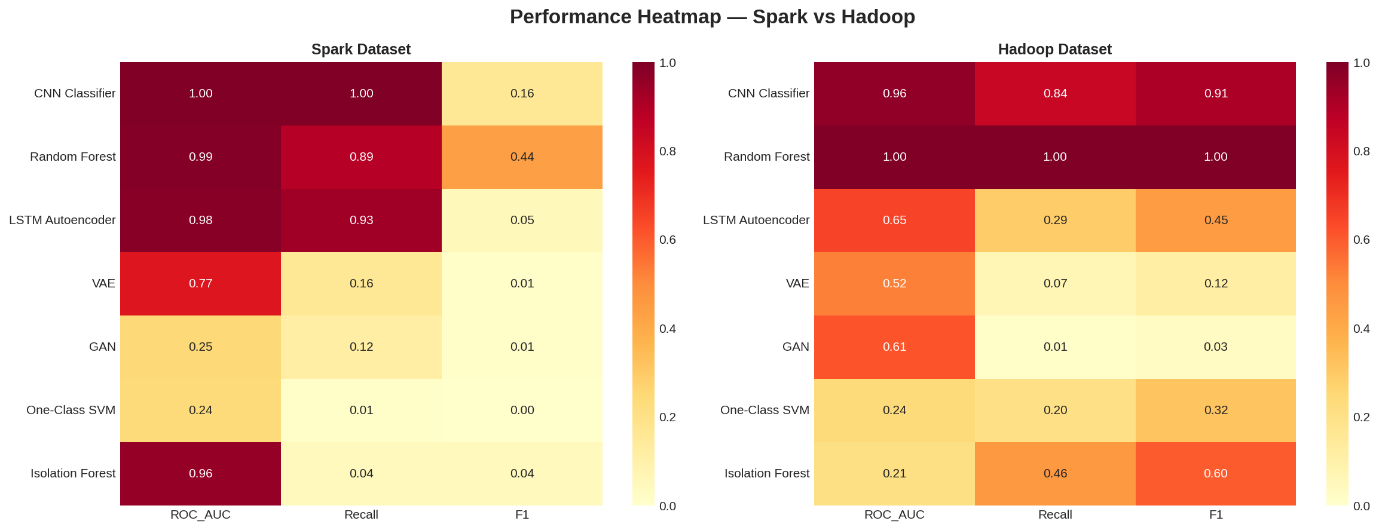
\includegraphics[width=3.125in,height=1.19792in]{./media/8ed9ab2b6d3e467bd8b4023ea365d50795af3823.png}

Fig. 35. Overall performance matrix --- Spark vs. Hadoop across all
evaluated models.

Three key patterns emerge. First, the "HDFS illusion": nearly every
model performs exceptionally well on HDFS, suggesting the
anomaly-detection problem is largely solved---an impression that does
not generalize. Second, the Spark reality check: the complex,
overlapping nature of Spark execution logs collapses F1-scores below
0.50 for almost every model despite strong ROC-AUC values. Third, the
generative struggle: while theoretically advantageous for removing
manual feature engineering, Generative AI consistently underperforms
across all environments, peaking at F1 = 0.7946 on HDFS and failing on
Spark and Hadoop.

\textsc{VI. CONCLUSION AND FUTURE WORK}

This paper presented a comparative study of Traditional ML, Deep
Learning, and Generative AI for automated log anomaly detection across
HDFS, Apache Spark, and Hadoop. The findings reveal a clear trade-off
between accuracy and functional autonomy: traditional supervised
classifiers achieve near-perfect F1-scores on structurally consistent
datasets but depend on manual feature engineering; supervised deep
sequence models remove this dependency while matching accuracy, yet
degrade under Spark\textquotesingle s noise and concurrency; and
Generative AI, despite consistently high ROC-AUC, achieves lower
F1-scores overall, establishing only a baseline capability for zero-day
anomaly discovery rather than outright superiority over supervised
approaches.

Future work will explore dynamic thresholding (e.g., extreme value
theory) to reduce false positives in generative models, online
incremental learning for concept-drift mitigation, fine-grained parsing
of variable log fields, and hybrid neuro-symbolic frameworks combining
ensemble robustness with generative flexibility.

\textsc{ACKNOWLEDGMENT}

The author thanks Prof. Dr. Imran Ihsan for his supervision and guidance
throughout this research.

\textsc{REFERENCES}

{[}1{]} J. Zhu, S. He, P. He, J. Liu, and M. R. Lyu, "Loghub: A large
collection of system log datasets for AI-driven log analytics," in Proc.
IEEE 34th Int. Symp. Software Reliability Engineering (ISSRE), 2023, pp.
355--366.

{[}2{]} W. Meng et al., "LogAnomaly: Unsupervised detection of
sequential and quantitative anomalies in unstructured logs," in Proc.
28th Int. Joint Conf. Artificial Intelligence (IJCAI), 2019, pp.
4739--4745.

{[}3{]} P. He, J. Zhu, Z. Zheng, and M. R. Lyu, "Drain: An online log
parsing approach with fixed depth tree," in Proc. IEEE Int. Conf. Web
Services (ICWS), 2017, pp. 33--40.

{[}4{]} M. Du, F. Li, G. Zheng, and V. Srikumar, "DeepLog: Anomaly
detection and diagnosis from system logs through deep learning," in
Proc. ACM SIGSAC Conf. Computer and Communications Security, 2017, pp.
1285--1298.

{[}5{]} X. Zhang et al., "Onion: Identifying incident-indicating logs
for cloud systems," in Proc. 29th ACM Joint Meeting European Software
Engineering Conf. and Symp. Foundations of Software Engineering
(ESEC/FSE), 2021, pp. 1253--1263.

{[}6{]} W. Xu, L. Huang, A. Fox, D. A. Patterson, and M. I. Jordan,
"Detecting large-scale system problems by mining console logs," in Proc.
ACM SIGOPS 22nd Symp. Operating Systems Principles (SOSP), 2009, pp.
117--132.

{[}7{]} F. T. Liu, K. M. Ting, and Z. H. Zhou, "Isolation forest," in
Proc. 8th IEEE Int. Conf. Data Mining (ICDM), 2008, pp. 413--422.

{[}8{]} Q. Lin, H. Zhang, J. G. Lou, Y. Zhang, and X. Chen, "Log
clustering based problem identification for online service systems," in
Proc. 38th Int. Conf. Software Engineering Companion (ICSE-C), 2016, pp.
102--111.

\end{document}
